\begin{apendicesenv}
  
  \chapter{Processo de Engenharia de Requisitos}
  
    \begin{figure}[!htbp]
      \centering
      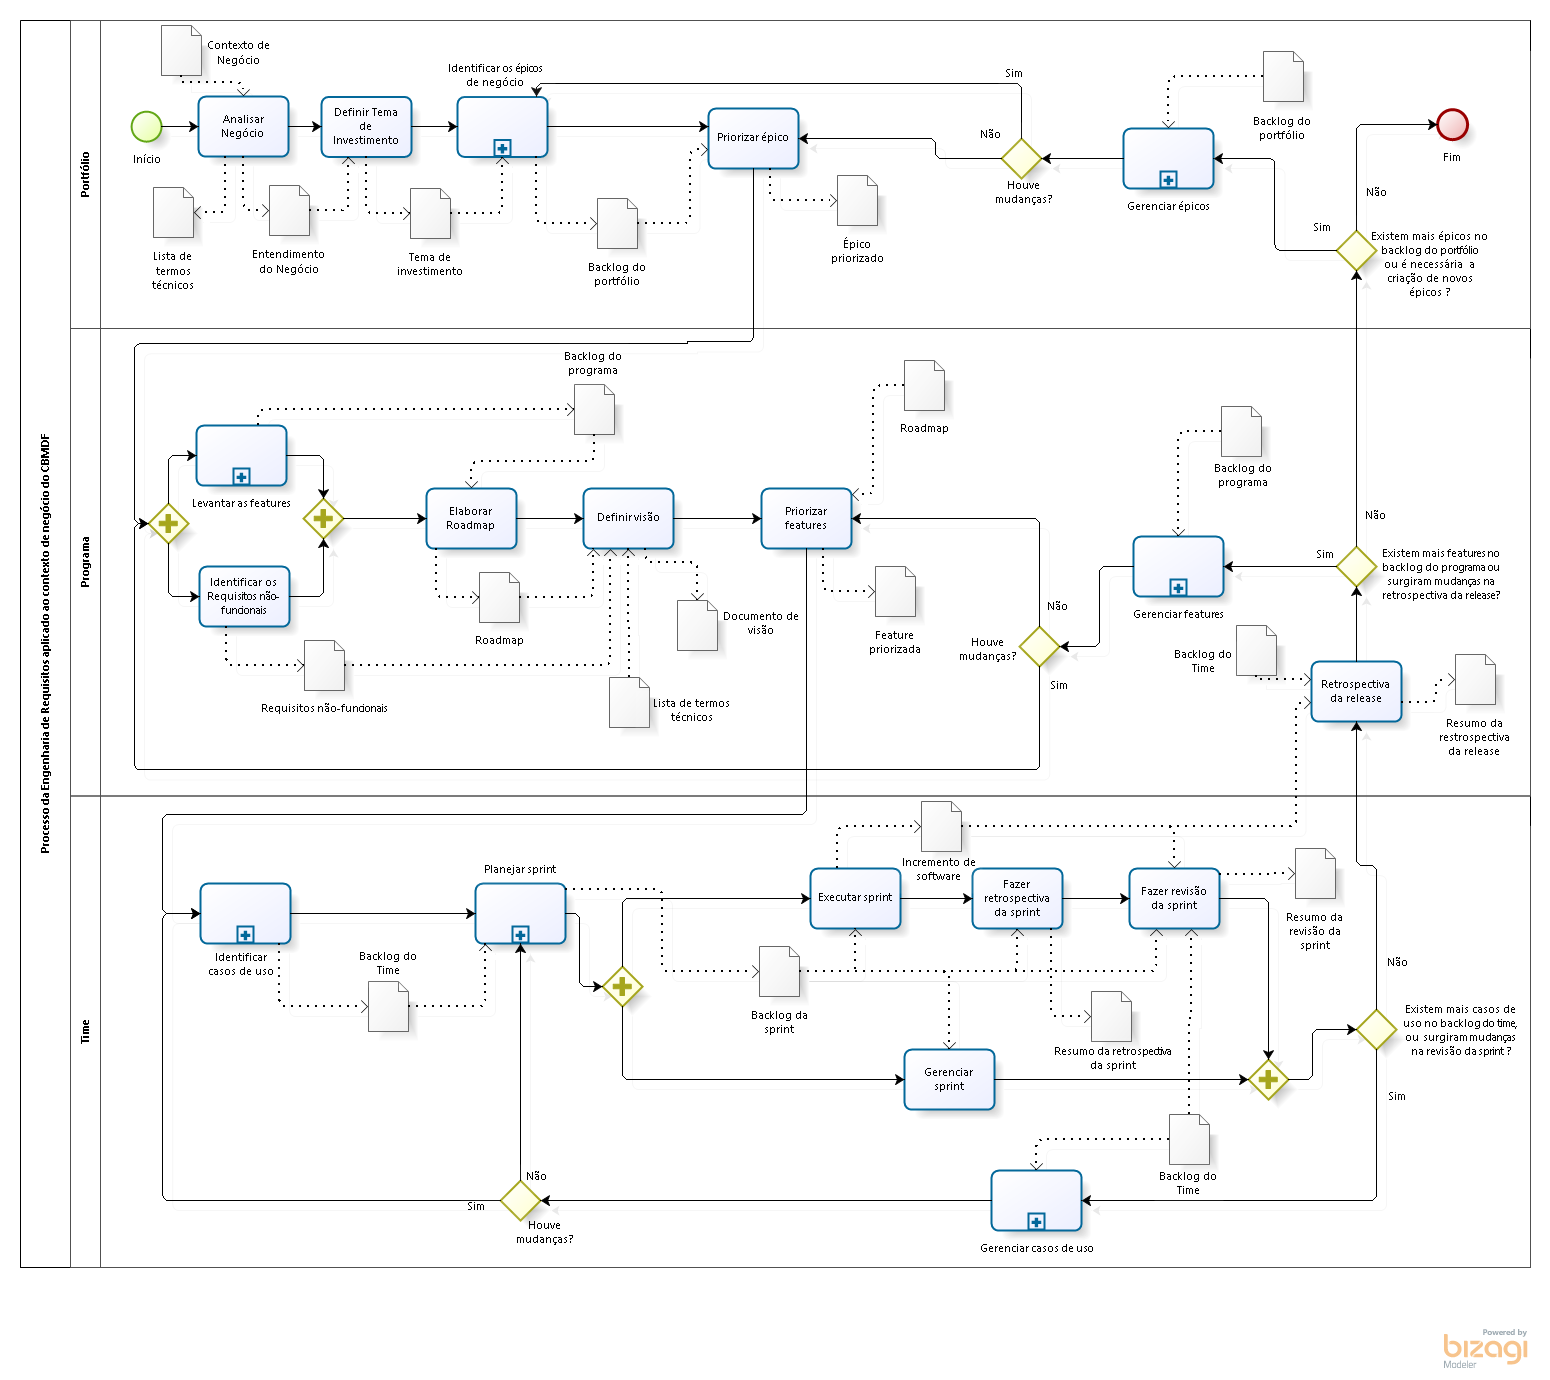
\includegraphics[scale=0.46, angle = 90]{figuras/project_big_picture}
      \caption[Modelo do processo de Engenharia de Requisitos]
	  {Modelo do processo de Engenharia de Requisitos: \textit{Big Picture} do projeto.}
      \label{project_big_picture}
    \end{figure}
  
  \chapter{Documento de visão}
	{\centering
	\textbf{Corpo de Bombeiros Militar do Distrito Federal}

	\textbf{Documento de visão para o sistema de gerenciamento de viaturas}

	\textbf{2015}

	}
	\textbf{Histórico de Revisões}
	\begin{table}[h]
	\centering
	\label{my-label}
	\begin{tabular}{|l|l|l|l|}
	\hline
	Data & Revisão & Descrição & Autor \\ \hline
	14/06/2015 & 1.0 & Versão Inicial & João Paulo \\ \hline
	22/06/2015 & 1.1 & Adição dos RNF & João Paulo \\ \hline
	     &         &           &       \\ \hline
	\end{tabular}
	\caption{Histórico de Revisões}
	\end{table}
  
	\section{Introdução}
		\subsection{Propósito}
Este documento define as estratégias utilizadas para nortear o desenvolvimento do projeto, as necessidades do usuário e envolvidos no projeto,
		\subsection{Resumo da solução}
A solução se apresenta sob a forma de uma aplicação que funcionará na intranet do Corpo de Bombeiros Militar do Distrito Federal, e fornecerá subsídios para o correto gerenciamento das viaturas e pessoal relacionado à esse contexto. A aplicação será desenvolvida a partir das necessidades do cliente, sem conexão com um sistema legado.
	\section{Descrição do Usuário}
		\subsection{Ambiente de Usuário}
Os usuários são funcionários do Corpo de Bombeiros Militar do Distrito Federal e utilizarão o sistema nas Unidades.
		\subsection{Principais necessidades do Usuário}
Para o usuário é primordial organizar e automatizar a gestão de viaturas e motoristas, desde o Departamento de Gestão Veicular até o controle de viaturas e motoristas nas unidades.
	\section{\textit{Stakeholders}}
Os envolvidos no projeto seja no desenvolvimento, na aquisição ou no uso da aplicação final são stakeholders. No contexto de desenvolvimento do sistema de gestão de viaturas do CBM-DF temos os seguintes \textit{stakeholders}:
\begin{itemize}
 \item Equipe de desenvolvimento;
 \item Bombeiros do CBM-DF;
 \item Funcionários do DGV;
\end{itemize}
	\section{Resumo do Produto}
Nesta seção serão definidas características do produto.
		\subsection{Perspectiva do Produto}
Espera-se do produto que melhore a gestão de viaturas e motoristas no CBM-DF, facilitando consultas, relatórios, verificações e utilização.
		\subsection{Intenção do Produto}
O sistema de gerenciamento automatizará as atividades que hoje são feitas à mão e são arquivadas sob forma de planilhas eletrônicas. Os usuários do DGV e Unidades utilizarão o sistema afim de automatizar suas atividades.
		\subsection{Resumo das Capacidades}
O sistema de Gerenciamento de Viaturas e Motoristas do CBM-DF permitirá o gerenciamento de viaturas, criando viaturas nos sistemas, alocando viaturas às unidades e modificando os estados das viaturas. Também serão gerenciados os motoristas, adicionando os mesmo no sistema, modificando dados do motorista, alocando motoristas em escalas e em viaturas.
	\section{Funcionalidades do Produto}
As funcionalidades são um conjunto de características e comportamentos que o sistema deve conter para resolver o problema e as necessidades do cliente.
		\subsection{\textit{Feature} 1: Gerenciamento das missões das unidades}
Esta funcionalidade compreenderá comportamentos que permitirão ao usuário fazer gerenciamento de missões atribuindo viaturas a elas e gerar relatórios do trabalho registrado no sistema.
		\subsection{\textit{Feature} 2: Gerenciamento dos dados de abastecimento das viaturas}
Esta funcionalidade facilitará o gerenciamento dos abastecimentos, visto que o usuário, propriamente dotado de autorização, poderá inserir dados de um abastecimento juntamente com o recibo do próprio. Além disso a funcionalidade garante a geração de relatórios dos dados aqui contidos.
		\subsection{\textit{Feature} 3: Gerenciamento dos motoristas das unidades}
Esta funcionalidade será empregada tanto para o DGV quanto para as Unidades, com a finalidade de gerenciar o motorista desde o cadastro do próprio no sistema quanto na alocação em uma escala e missões, além de compreender a geração de relatórios desse assunto.
		\subsection{\textit{Feature} 4: Gerenciamento das viaturas do CBM-DF}
Esta funcionalidade compreende as necessidades do usuário de gerenciar viaturas desde o cadastro e alocação, até o desígnio para as missões. Aterações de estado e geração de relatórios deste assunto estão aqui contidos.
	\section{Requisitos não-funcionais}		
Requisitos não-funcionais são regras que não necessariamente são funcionalidades do sistema, mas o sistema deve estar em conformidade com 
\begin{itemize}
 \item O sistema deve ficar online 24/7;
 \item O sistema deve estar disponível na Intranet do CBMDF;
 \item O sistema deve possuir uma interface autoexplicativa;
 \item O sistema deve fornecer informações mais detalhadas sobre o funcionamento de suas funcionalidades, quando necessário;
 \item O sistema deve possuir uma versão mobile, com determinadas funcionalidades, na plataforma Android;
 \item O sistema deve manter uma cópia local e atualizada de determinados dados, em sua versão mobile, provenientes do banco de dados do sistema;
 \item O sistema deve exigir uma verificação de identidade para que o acesso seja liberado.
\end{itemize}
	\section{Documentação dos Requisitos}
		\subsection{Glossário}
Neste item definimos termos a fim de tornar comum o entendimento dos envolvidos.
\begin{itemize}
 \item \textit{Stakeholder}: Envolvido com a produção,utilização ou gerenciamento do projeto.
 \item CBM-DF: Corpo de Bombeiros Militar do Distrito Federal.
 \item DGV: Departamento de Gestão Veicular.
 \item Chamado: Demanda criada por uma ligação de telefone e passada pela central para alguma unidade.
 \item Missão: Atividade dos bombeiros das unidades.
\end{itemize}
\end{apendicesenv}
